\subsubsection{Architecture}

\par{Table \ref{tab:phi_arch} contains the main hardware characteristics of the Xeon Phi device.}

\begin{table}[!h]
    \centering
    \begin{tabular}{| l | l | l | l |}
    \hline
    \# cores & 60(in-order) \\ \hline
    clock speed & 1.053 GHz \\ \hline
    vector unit & 512-bit \\ \hline
    L1 & 32KB(data)+32KB(instructions) 64KB total\\ \hline
    L2 & 512KB(data+instructions)\\ \hline
    \end{tabular}
    \caption{Xeon Phi characteristics.}
    \label{tab:phi_arch}
\end{table}

\par{Every core contains vector arithmetic unit(executing SIMD vector instructions). It fits 8 double precision 
    floating point numbers, or 16 single precision floating point numbers. Each core can issue a single vector instruction per
    cycle\cite{opencl_phi}(this execution looks similar to an Nvidia GPU \emph{warp}), so vector instructions issued by 
    different threads in the same core are sequentialized, they do not execute in parallel(at the same cycle).}

\par{L1 cache misses have a latency of 15-30 cycles and access to L1 cache has a latency of 1 cycle. Each core has a L2 cache,
    combined all these L2 cache is a total 30MB of L2 cache in the device, miss latency for this type of memory is 500-1000 
    cycles\cite{opencl_phi,phi_specs}.}

\par{Also Xeon Phi provides a high speed interconect between L2 caches and the memory subsystem, a simple automatic hardware 
    prefetcher to L2 and each core can execute 4 hardware threads simultaneously, 240 threads in total. These threads help to hide 
    instruction and memory latency\cite{opencl_phi}.}

\par{OpenCL hides most of this detail from the programmer, figure \ref{PhiArch} shows a global view of the Intel Xeon Phi 
    architecture\cite{opencl_phi}.}

\begin{figure}[!h]
    \centering
    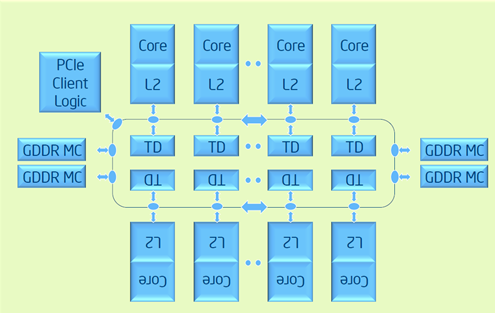
\includegraphics[width=0.4\textwidth]{figures/phi_arch.png}
    \caption{Intel Xeon Phi architecture\cite{opencl_phi}.}
    \label{PhiArch}
\end{figure}

\subsubsection{Mapping}
\begin{itemize}
    \item A \emph{work group} is the smallest task being scheduled on the threads\cite{opencl_phi}.
    \item \emph{Kernels} execute concurrently on multiple \emph{work items} in the SIMD units of every core\cite{opencl_phi_opt}.
    \item Each \emph{work group} is assigned to one thread that loops over all \emph{work items} within the \emph{work group} 
        with SIMD. Thus you have parallelism at the \emph{work group} level (vector instructions) and parallelism between 
        \emph{work groups} (threading)\cite{opencl_phi_opt}.
    \item At initialization time the Intel OpenCL driver creates 240 software threads and pins them to the hardware threads, then
        when you call \emph{clEnqueueNDRange()}, the intel driver schedules the \emph{work groups} of the current \emph{NDRange}
        into the 240 threads\cite{opencl_phi}.
    \item The OpenCL compiler implicitely vectorize the \emph{work group} routine based on dimension zero loop.
    \item The recommended work-group size for kernels is multiple of 16, which equals the SIMD width for the float and int data 
        type. The automatic vectorization module packs the work-items into SIMD packets of 16 items (for double as well), and 
        processed the rest (“tail”) of the work-group in a scalar way. In other words, a work-group with the size of 2*SIMD\_WIDTH 
        executes faster than, the one with the size of 2* SIMD\_WIDTH-1\cite{opencl_phi_opt,opencl_phi}.
    \item Non-uniform branching at dimension 0 the \emph{NDRange} is executed by flattening the code via predication and 
        ultimatelly executing both path of the branch and then apply masks, thus the usage of non-uniform branching is penalized by 
        a high overhead in the execution of the \emph{kernel}\cite{opencl_phi}.
    \item Using OpenCL \emph{local memory} does not provide any benefit on the Intel Xeon Phi. OpenCL \emph{local memory} is 
        allocated on the regular GDDR memory(\emph{global memory}) and is supported by the cache system like any other memory. 
        Therefore, it introduces additional overhead in terms of redundant data copy and management\cite{opencl_phi}.
    \item The combination of \emph{kernel} with barriers and \emph{work groups} nondivisible by 16, results in the execution of a
        scalar \emph{kernel}.
\end{itemize}

\begin{figure}[!h]
    \centering
    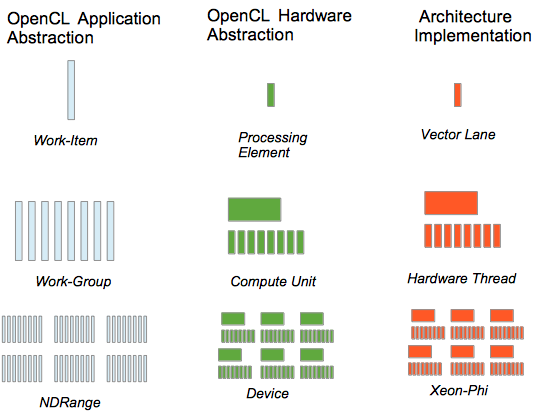
\includegraphics[width=0.4\textwidth]{figures/phi_model.png}
    \caption{OpenCL mapping for Intel Xeon Phi.}
    \label{PhiModel}
\end{figure}

\par{Figure \ref{PhiModel} shows a summary of the mapping of OpenCL concepts into the Intel Xeon Phi co-processor, figure 
    \ref{PhiDeviceInfo} shows the output of an OpenCL information request to the OpenCL run-time, it shows 236 
    \emph{compute units}(one per thread), the size of \emph{local memory} 32KB that match with the total amount of memory for L1 cache and
    the 6GB of total \emph{global memory} that matches with the amount of RAM available on the Intel Xeon Phi. In this context is 
    safe to assume that private memory on the Intel Xeon Phi is implemented via hardware registers.} 

\begin{figure}[!h]
    \centering
    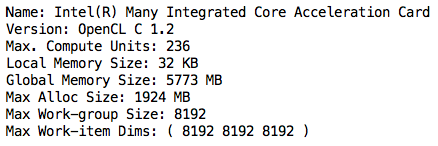
\includegraphics[width=0.45\textwidth]{figures/phi_device_info.png}
    \caption{Intel Xeon Phi device information.}
    \label{PhiDeviceInfo}
\end{figure}



